% ----------------------------------------------------------------------------------------------------------
% Die Grundlagen
% ----------------------------------------------------------------------------------------------------------
\section{Grundlagen}\label{grundlagen}
	Um die Vorgänge und die Funktionsweise des Lasertriangulationssensors genau zu verstehen, sollen zuvor einige Grundlagen für den Lösungsansatz erläutert werden. Angefangen wird mit der mathematischen Grundlage, um die internen Berechnungen nachzuvollziehen. Danach wird der Algorithmus besprochen, der zum Finden der Laserlinien-Pixel benutzt wird. Da dabei gewisse Bibliotheken mit Python zum Einsatz gekommen sind, sollen diese im ersten Schritt kurz erwähnt werden.
	
	\subsection{Bibliotheken}
	Der Lasertriangulationssensor wurde vor Allem mit OpenCv und ROS2 entwickelt. OpenCv bietet die perfekte Unterstützung für die benötigte Bildverarbeitung. Diverse Funktionen, um Bilder zu bearbeiten, zur Kamerakalibrierung und zum Errechnen der Ebenengleichung sind in OpenCv implementiert. \newline
	ROS2 kümmert sich um die Automatisierung und den generellen Ablauf eines Scanvorgangs. In dem Forschung- und Entwicklungs-Projekt mit RINNTECH wird zusätzlich auch ROS2 als übergeordnetes System genutzt. Deshalb war ROS2 auch eine Anforderung an das Projekt. Die vorher benutzte RGB-D-Kamera Intel RealSense ist ebenfalls in der Lage über ROS2 angesprochen zu werden. Da der OpenSource-Lasertriangulationssensor diese ersetzten soll, ist die Verwendung von ROS2 ein logischer Schritt. \newline
	Erwähnenswert  ist ebenfalls die junge Bilbiothek Open3D. Sie wird benötigt, um mit Punktewolken zu arbeiten.
	
	\subsection{Der grundlegende Aufbau}
	Der grundlegende Aufbau orientiert sich an dem Lösungsansatz. Notwendig sind dafür nur ein Linienlaser und eine Kamera. Zuerst wurde für einen Prototyp zum Testen eine Webcam verwendet, später eine Industriekamera. Ausschlaggebend zum Funktionieren des theoretischen Lösungsansatz ist, dass die Kamera einen Linienversatz aufnehmen kann. Um das zu erreichen, werden Kamera und Laser in einem gewissen Winkel zueinander gesetzt. Durch die Perspektive der Kamera entsteht der Linienversatz. Dabei ist egal, ob die Kamera von oben auf das Objekt zeigt und der Laser schräg sitzt oder andersrum. Die Lasertriangulationssensoren aus der Industrie weisen zumeist den Aufbau aus Abb. (\ref{fig:lasertriangulation}) auf. Abb. (\ref{fig:lasertriangulation_position}) zeigt den anderen Aufbau, wobei der Linienversatz aufgezeigt wird.
	
	\newpage
	
	\begin{figure}[h]
		\centering
		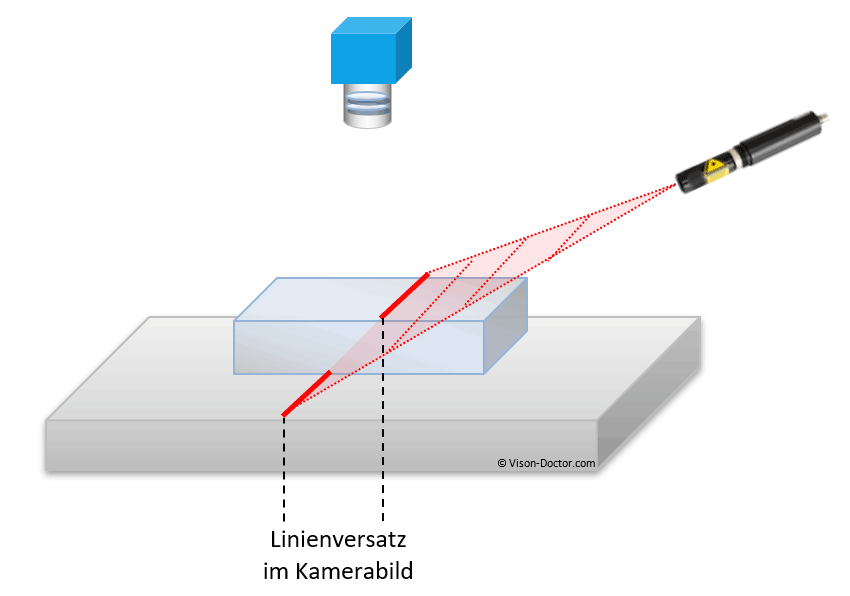
\includegraphics[width=0.6\linewidth]{img/grundlagen/lasertriangulation_2}
		\caption{Positionen bei der Lasertriangulation}
		\captionsource{Abbildung entnommen aus \citep{noauthor_prinzip_nodate}}
		\label{fig:lasertriangulation_position}
	\end{figure}
	
	Die Entwicklung lässt sich in zwei Abschnitte aufteilen. Der erste Abschritt ist die Erarbeitung des Lasertriangulationssensors. Dessen Aufgabe ist es, eine aufgenommene Laserlinie in eine korrekte Punktewolke umzusetzen. Danach muss es dem Sensor ermöglicht werden, sich über das Objekt zu bewegen. Möglich ist auch, dass Objekt unter dem Sensor durch zu bewegen. \newline
	Wichtig ist, dass die Kamera und Laser in einem Winkel zueinander über dem Objekt angebracht sind (Abb. (\ref{fig:lasertriangulation}), (\ref{fig:lasertriangulation_position})). Dabei ist ausschlaggebend, dass Kamera und Laser fest angebracht sind und sich zueinander nicht bewegen. Nur der ganze Sensor ist bewegbar, dabei bleiben dann Kamera und Laser zueinander in der gleichen Position.
	\label{chap:grundlegender_aufbau}
	
	\subsection{Pinhole Camera Model}
	Wenn eine Kamera ein Bild aufnimmt, ist das eine Abbildung eines dreidimensionalen Raumes (die Szene) auf eine zweidimensionale Ebene (das Bild). Der Lasertriangulationssensor soll diesen Prozess umgekehrt realisieren. Die Grundlage ist das aufgenommene Bild. Ein Bild besteht aus Pixeln. Ausgehend von diesem, soll der dreidimensionale Raum digital abgebildet werden. Das bedeutet, dass für jeden Pixel eine definierte Abbildung im dreidimensionalen Raum gefunden werden muss. Für diese Abbildungen ist in OpenCv das \textbf{Pinhole Camera Model} implementiert. Hier wird die Kamera digital als eine Lochkamera begriffen. \newline
	\begin{figure}[h]
		\centering
		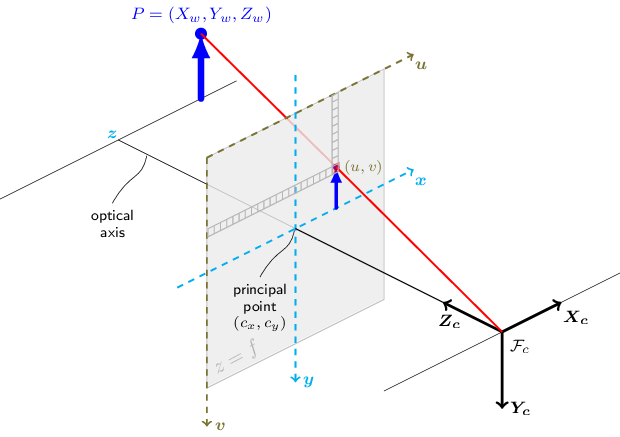
\includegraphics[width=0.7\linewidth]{img/grundlagen/pinhole_camera_model.png}
		\caption{Pinhole Camera Model}
		\captionsource{Abbildung entnommen aus \citep{noauthor_opencv_nodate-2}}
		\label{fig:pinhole-camera-model}
	\end{figure}
	In Abb. (\ref{fig:pinhole-camera-model}) ist dieses Modell dargestellt. An dem optischen Zentrum orientiert sich das Kamera-Koordinatensystem (\( F_c \)). Dabei wäre das optisches Zentrum bei einer Lochkamera die Lochblende oder bei einer herkömmlichen Kamera der optische Sensor. Wenn mit einer Lochkamera ein Bild aufgenommen wird, erscheint die Abbildung auf dem Kopf gespiegelt auf einer Bildebene. Das hat physikalische Gründe. Das Pinhole Kamera Model ist aber rein digital. So muss die Bildebene nicht hinter dem optischen Sensor sein. Sie wird zwischen dem optischen Zentrum und der Abbildung im dreidimensionalen Raum dargestellt. So kann ein Punkt in der Szene als Vektor begriffen werden, der durch die Bild-Ebene einen Pixel definiert und zum optischen Zentrum führt \citep[vgl.][]{dawson-howe_simple_1994}. Zu sehen in Abb. (\ref{fig:pinhole-camera-model}) als die rote Linie. In diesem Fall ist das Bild und die genaue Position eines Pixels mit u und v bekannt. Das Ziel ist es, die dazugehörige 3D-Koordinate (P) zu erhalten.
	\newpage 
	
	\subsection{Mathematische Grundlage}
	Die Grundlage für die Berechnungen mit den Pixeln aus einem Bild ist die folgende Formel:
	
	\begin{equation}
	s \; p_{pix} = A \begin{bmatrix} R|t \end{bmatrix} p_w
	\label{eq:basic_trans}
	\end{equation}
	
	Sie beschreibt die Projektion eines 3D-Punktes in eine Szene zu einem Punkt in der Bild-Ebene. Hierbei ist \( p_{pix} \) der Pixel im Bild. \( p_w \) ist die Welt-Koordinate, welche gesucht wird. \( A \) ist die Kamera-Matrix.\( \begin{bmatrix} R|t \end{bmatrix} \) ist eine Rotation und Translation und beschreibt eine Transformation vom Kamerakoordinatensystem zum Weltkoordinatensystem. Die genaue Entstehung der Formel beschreibt OpenCv in \citep[vgl.][]{noauthor_opencv_nodate-2}. Kamera-Matrix, Rotation und Translation sind hierbei neu. Die genaue Bedeutung wird in dem Kapitel \ref{chap:kalibierung} Kalibrierung genannt. Zum Verstehen der Formel ist hier nur wichtig, dass diese durch eine Kamerakalibrierung herausgefunden werden können \citep[vgl.][]{dawson-howe_simple_1994}. Die Variablen sind also bekannt. Kamera-Matrix und Rotation sind beide jeweils 3x3 Matrizen. Die Translation wird durch einen Vektor (3x1) beschrieben. 
	
	\begin{equation}
	s \; \begin{bmatrix}
	u \\ 
	v \\ 
	1
	\end{bmatrix} = \begin{bmatrix}
	f_x & 0 & c_x \\
	0 & f_y & c_y \\
	0 & 0 & 1
	\end{bmatrix} \times \begin{bmatrix}
	r_{11} & r_{12} & r_{13} & t_1 \\ 
	r_{21} & r_{22} & r_{23} & t_2 \\ 
	r_{31} & r_{32} & r_{33} & t_3
	\end{bmatrix} \times \begin{bmatrix}
	X \\ 
	Y \\ 
	Z \\
	1
	\end{bmatrix}
	\label{eq:basic_trans_complete}
	\end{equation}
	
	In der Formel (\ref{eq:basic_trans_complete}) wird dies noch einmal genauer gezeigt. Bekannt sind also \( p \), \( A \) und \( \begin{bmatrix} R|t \end{bmatrix} \). Unbekannte Variablen sind \( s \) der Scale-Factor und \( p_w \) die Weltkoordinate.
	
	\subsubsection{Koordinaten-Transformationen}
	Um den 3D-Punkt im Weltkoordinatensystem anhand eines Pixels zu errechnen, wird die grundlegende Formel umgestellt. Die folgende Abbildung (\ref{fig:pinhole-camera-model_transformations}) zeigt nochmal das Pinhole Camera Model und verdeutlicht dabei die angewandten Transformationen.
	
	\begin{figure}[h]
		\centering
		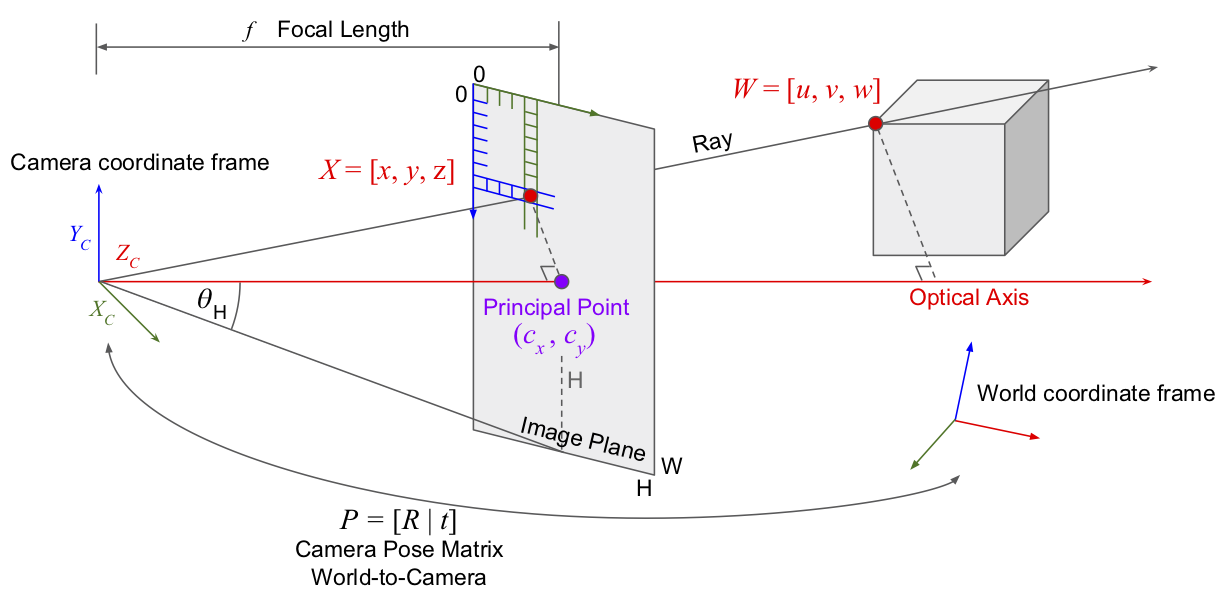
\includegraphics[width=0.9\linewidth]{img/grundlagen/pinhole_camera_model_2.png}
		\caption[Transformationen]{Transformationen im Pinhole Camera Model}
		\captionsource{Abbildung entnommen aus \citep{pinhole_camera_model}}
		\label{fig:pinhole-camera-model_transformations}
	\end{figure}
	
	Das Ziel ist es, den 3D-Punkt (in Abb. (\ref{fig:pinhole-camera-model_transformations}) \( W \)) im Weltkoordinatensystem zu errechnen. Die Rotation (R) und Translation (t) werden für die Umrechnung in das Kamerakoordinatensystem benötigt. Das sind die sogenannten extrinsischen Parameter. In Abb. (\ref{fig:pinhole-camera-model_transformations}) wird diese Transformation unter \( P \) der \textbf{Camera Pose Matrix} dargestellt. \newline
	Die Kamera-Matrix beschreibt die Transformation zur Bild-Ebene bzw. den Pixelkoordinatensystem. Die Matrix enthält die sogenannten intrinsischen Parameter. Das ist die in Abb. (\ref{fig:pinhole-camera-model_transformations}) gezeigte \textbf{Focal Length} \( f \), welche den Abstand vom Kamera-Koordinatensystem zur Bild-Ebene beschreibt. Hinzu kommt der \textbf{Principal Point}. Dieser befindet sich in dem Zentrum der Bild-Ebene. Beides zusammen ergibt die gezeigte Matrix aus (\ref{eq:basic_trans_complete}) \citep[vgl.][]{noauthor_opencv_nodate-1}. Letztendlich wird damit die Umrechnung vom Kamerakoordinatensystem (in Abb. (\ref{fig:pinhole-camera-model_transformations}) \textbf{Camera coordinate frame}) zur Bild-Ebene (in Abb. (\ref{fig:pinhole-camera-model_transformations}) \textbf{Image Plane}) dargestellt. \newline 
	Es ist möglich, einen Pixel im Bild auszuwählen und mithilfe dieser Parameter den entsprechenden Punkt im Weltkoordinatensystem errechnen. Dazu muss die Formel (\ref{eq:basic_trans}) nach dem Punkt im Weltkoordinatensystem umgestellt werden.
	
	\begin{equation}
	\begin{aligned}
	\begin{bmatrix} A \end{bmatrix} \begin{bmatrix} R|t \end{bmatrix} p_w &= s \; p_{pix} \\
	\begin{bmatrix} R|t \end{bmatrix} p_w &= s \begin{bmatrix} A \end{bmatrix}^{-1} p_{pix} \\
	\begin{bmatrix} R \end{bmatrix} p_w &= s \begin{bmatrix} A \end{bmatrix}^{-1} p_{pix} - t \\
	p_w &= s \begin{bmatrix} R \end{bmatrix}^{-1} \begin{bmatrix} A \end{bmatrix}^{-1} p_{pix} - \begin{bmatrix} R \end{bmatrix}^{-1} t \\
	p_w &= s \; \vec{a} - \vec{b} \\
	wobei: \quad \vec{a} & = \begin{bmatrix} R \end{bmatrix}^{-1} \begin{bmatrix} A \end{bmatrix}^{-1} p_{pix} \\
	\vec{b} &= \begin{bmatrix} R \end{bmatrix}^{-1} t
	\end{aligned}
	\label{eq:pixel_zu_welt}
	\end{equation}
	
	Diese Gleichung ist die Grundlage der Errechnung von 3D-Informationen. \( \vec{a} \) und \( \vec{b} \) dienen zur Vereinfachung. Wenn \( \begin{bmatrix} R \end{bmatrix} \), \( \begin{bmatrix} A \end{bmatrix}^{-1} \) und \( p_{pix} \) miteinander verrechnet werden entsteht ein Vektor (\( \vec{a} \)). Genauso entsteht aus\( \begin{bmatrix} R \end{bmatrix}^{-1} \) und \( t \) der Vektor (\( \vec{b} \)). Zusätzlich beschreibt \( s \; \vec{a} - \vec{b} \) eine Gleichung für eine Linie im dreidimensionalen Raum. Damit stellt sie den beschriebenen Vektor in \citep[vgl.][S. 3]{dawson-howe_simple_1994} und die rote Linie in Abb. (\ref{fig:pinhole-camera-model}) und (\ref{fig:pinhole-camera-model_transformations}) dar. \newline
	Der neue Ausgangspunkt ist die errechnete Weltkoordinate. Nach Aufgabenstellung sollen errechnete Koordinaten immer aus Sicht der Kamera dargestellt werden. Dazu wird die folgende Transformation benötigt. 
	
	Weltkoordinate zu Kamerakoordinate:
	\begin{equation}
	p_{cam} = \begin{bmatrix} R \end{bmatrix} \; p_{welt} + t
	\label{eq:welt_zu_kamera}
	\end{equation}
	
	Kamerakoordinate zur Weltkoordinate:
	\begin{equation}
	p_{welt} = \begin{bmatrix} R \end{bmatrix}^{-1} \; (p_{cam} - t)
	\label{eq:kamera_zu_welt}
	\end{equation}
	
	Anzumerken ist noch, dass \( s \) der Scale-Factor immer noch eine Unbekannte ist. Es scheint also, als ob die Gleichung (\ref{eq:pixel_zu_welt}) noch nicht lösbar sei. Sobald konkrete Werte ausgerechnet werden sollen, muss \( s \) bekannt sein. Das passiert zum ersten Mal beim Erstellen der Ebenengleichung für die Laser-Ebene bei der extrinsischen Kalibrierung. Dabei wird auch darauf eingegangen, wie \( s \) errechnet werden kann.  
	
	\newpage
	
	\label{chap:transformationen}
	\subsection{Bildverarbeitung}
	Bekannt sind nun gewisse Grundlagen, wie mit einem ausgewählten Pixel im Bild umgegangen werden kann. Die Rechnungen und Transformationen sollen aber nicht auf zufällige oder sogar alle Pixel im Bild angewandt werden. Sie sollen auf ganz bestimmte ausgewählte Pixel erfolgen. Und zwar ganz genau diese, die zur abgebildeten Laserlinie gehören. Die Laserlinie ist immer unser Ausgangspunkt für die 3D-Informationen. Alle anderen Pixel interessieren im Grunde nicht. \newline
	Pixel können einfach und eindeutig als Tupel benannt werden. Sie können als Punkt in einem zweidimensionalen Koordinatensystem begriffen und dann mit einem horizontalen und vertikalen Wert genau gekennzeichnet werden. Benötigte wird eine Menge an diesen Tupeln, für die gilt, dass sie Teil der Laserlinie im Bild sind. Mit diversen Methoden der Bildverarbeitung können diese Pixel herausgefunden und abgespeichert werden, um mit ihnen weiterarbeiten zu können. Das folgende Kapitel bildet somit einen Algorithmus ab, dessen Ziel es ist, ein Bild entgegenzunehmen und die Pixel der Laserlinie zurückzugeben. 
	
	\label{chap:bildverarbeitung}
	\subsubsection{Das Erkennen der Laserlinie}
	Der erste Schritt des Algorithmus muss sein, die Laserlinie im Bild zu erkennen. Ein wichtiges Kriterium dabei ist die Genauigkeit der ausgewählten Pixel. Jeder Pixel, der vom Algorithmus markiert wird, aber nicht zur eigentlichen Laserlinie gehört, wird in einem Fehler in der am Ende erstellten Punktewolke enden. Es wird also ein Punkt im Raum gezeigt, der nicht zur eingescannten Oberfläche passt. Dieser hängt dann beispielsweise in der Luft bzw. ist an einer Stelle im Koordinatensystem, wo sich eigentlich nichts befindet. Dieses sogenannte Rauschen soll möglichst gering sein. \newline
	Im Zuge einer umfangreichen Recherche zum Thema Lasertriangulation und OpenSource-Produzierten Laserlinienscannern wurde ein Paper von Bajpai und Perelman \citep[vgl.][]{bajpai_cross-platform_nodate}, die auch einen Laserlinienscanner entwickelt haben, als Grundlage gewählt. Nicht nur bei dem Finden der Laserlinie, auch in diversen anderen Schritten der Errechnung von 3D-Punkten aus den Laserlinien-Pixeln ist dieses Paper eine Grundlage und Hilfestellung. Gemäß der dort verwendeten Methodik wurde die Idee übernommen, zwei Bilder aufzunehmen. In einem ist der Laser angeschaltet, in dem anderen nicht. Wenn diese Bilder voneinander abgezogen werden, kommen im Grunde genau die Veränderungen hervor. Da sich nichts anderes im Bild verändern sollte, außer das Erscheinen der Laserlinie, wird diese genau aufgezeigt.
	Voraussetzung dafür ist, dass die Umgebung der zu scannenden Fläche gleich bleibt. Einwirkungen wären zum Beispiel Änderungen bei den Lichtverhältnissen bzw. bei der Beleuchtung oder auch eine Bewegung von Objekten zwischen der Aufnahme der zwei Bilder. Solche Einwirkungen würden in ungewolltem Rauschen enden oder sogar die Laserlinie falsch positionieren. Weitere Informationen hierzu befinden sich ebenfalls im Kapitel \ref{chap:probleme_schwierigkeiten} Probleme und Schwierigkeiten. Diese Anforderungen werden für den zu entwickelnden Laserlinien-Scanner akzeptiert. Ebenfalls sind es Anforderungen, die nicht direkt von der Software beeinflusst werden können. Sie sollten somit beim Aufbau des Scanners genauer beachtet werden und auf die Bildverarbeitung keinen Einfluss mehr haben dürfen. Die Methode ist außerdem ohne Probleme über OpenCv umsetzbar.
	
	\begin{figure}[h]
		\centering
		\subfloat[]{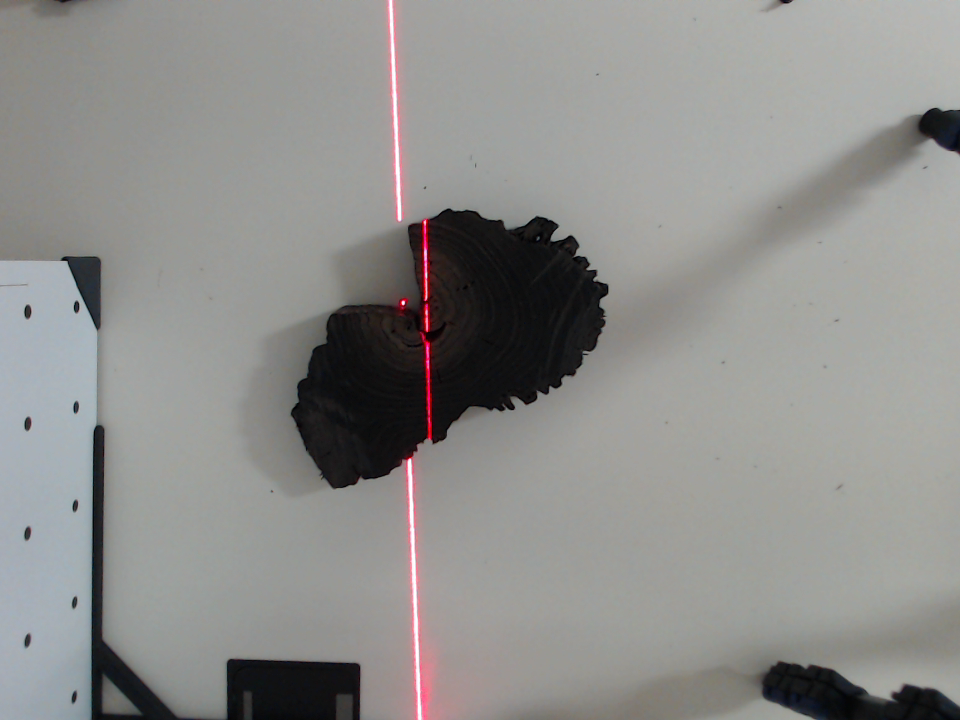
\includegraphics[width=0.325\linewidth]{img/hauptteil/bildverarbeitung/surface_img_1.png} \label{subfig:surface_laser}}
		\subfloat[]{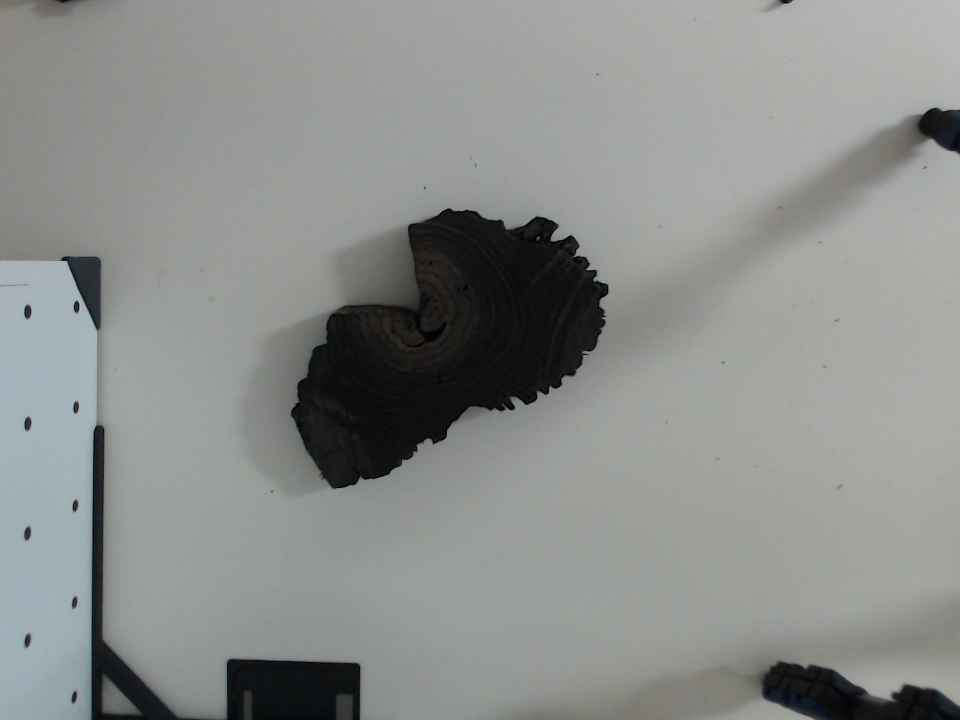
\includegraphics[width=0.325\linewidth]{img/hauptteil/bildverarbeitung/surface_img_0.png} \label{subfig:surface}}
		\subfloat[]{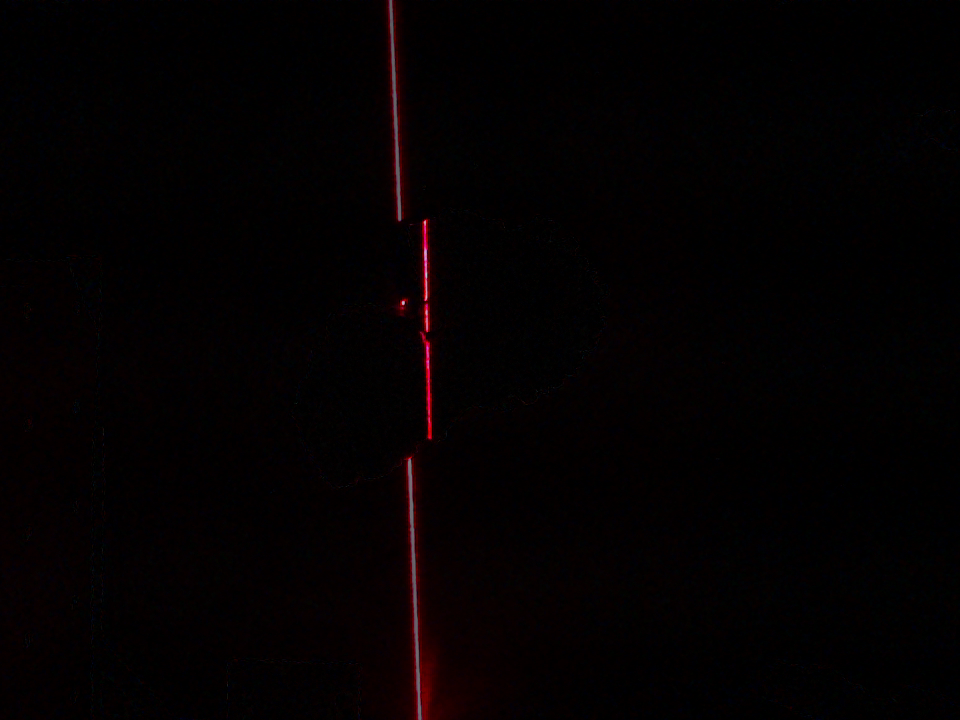
\includegraphics[width=0.325\linewidth]{img/hauptteil/bildverarbeitung/surface_diff.png} \label{subfig:surface_diff}}
		\caption{Subtraktion der Bilder}
		\label{fig:sub_imgs}
	\end{figure} 
	
	Festzuhalten ist damit, dass die Kamera zwei Bilder aufnehmen muss, eins Bild mit Laserlinie und ein Bild ohne. Das Bild ohne Laserlinie (\ref{subfig:surface}) wird dann von dem mit Laserlinie (\ref{subfig:surface_laser}) abgezogen. Der Algorithmus zum Finden der Laserlinien-Pixel arbeitet dann mit der Differenz (\ref{subfig:surface_diff}).
	
	\newpage
	
	\subsubsection{Umwandlung zu einem Grauwert-Bild}
	Für einen Menschen ist die Laserlinie jetzt schon auf einem Blick gut erkennbar. Ein Algorithmus braucht allerdings spezifische Informationen, um die Pixel auszuwählen. Auch die Pixel, die nicht eindeutig zur Laserlinie gehören sind nicht komplett schwarz mit einem RGB-Wert von (R=0, G=0, B=0). Einen kleinen für den Menschen zumeist nicht sichtbaren Unterschied in zwei nacheinander aufgenommenen Bildern wird es immer geben. 
	
	\begin{figure}[h]
		\centering
		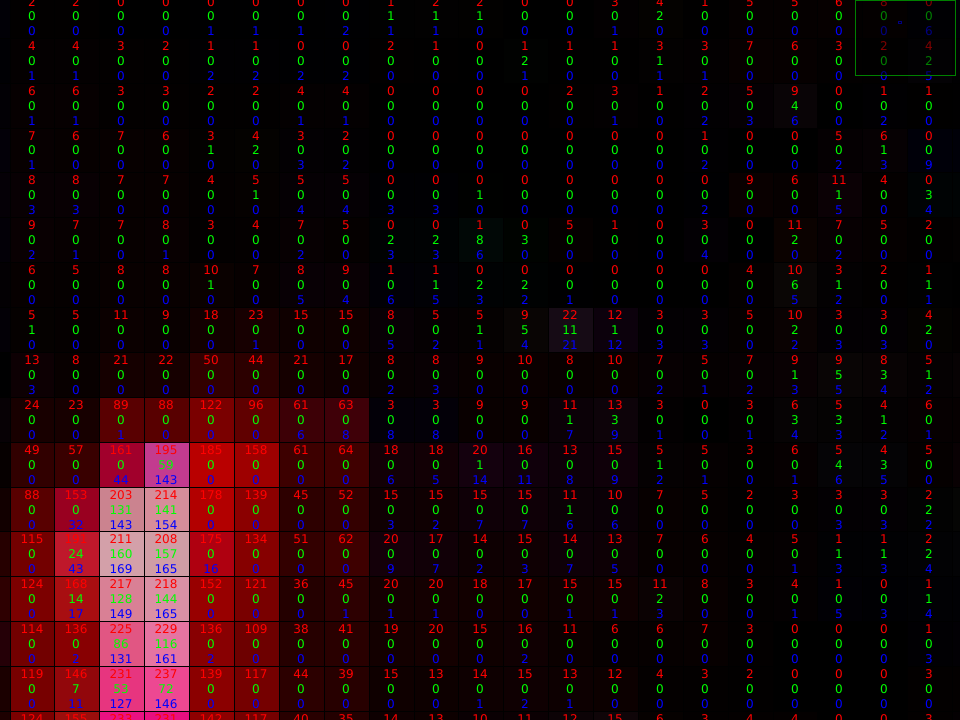
\includegraphics[width=0.75\linewidth]{img/hauptteil/bildverarbeitung/pixel_values.png}
		\caption[Pixel-Werte der Laserlinie]{Pixel-Werte in einem Ausschnitt aus \ref{subfig:surface_diff} am Rand der Laserlinie}
		\label{fig:pix_values}
	\end{figure} 
	
	Die Abbildung zeigt gut die Pixel der Laserlinie unten links. Die verschiedenen Farbbereiche sind stark vertreten, vor allem der Rote. Die Pixel, die kein Teil der Laserlinie sind, besitzen nur sehr schwache Werte in den drei Farbbereichen. Nach einer Regelung muss hier immer noch genau festgelegt werden, welche Pixel für die Laserlinie ausgewählt werden. Die Differenz von den zwei Bildern macht dies allerdings einfacher. Gleichbleibende Stellen zwischen den beiden Bildern wie zum Beispiel sehr helle Stellen oder auch andere rote Stellen sind in dem Differenz-Bild nicht mehr erkennbar. Ohne diesen Schritt wären diese womöglich nicht genau von der Laserlinie zu unterscheiden. \newline
	Als zweiter Schritt wird das Bild zu einem Grauwert-Bild konvertiert. Vorteil davon ist, dass nicht mehr der RGB-Wert mit drei eigenen Werten ausschlaggebend ist, sondern nur noch die Intensität, bzw. der Grauwert eines Pixels. Die jeweilige Intensität für einen Pixel berechnet OpenCv nach der folgenden Formel \cite[Vgl.][]{noauthor_opencv_nodate}:
	\begin{equation}
	Y = 0.299 \cdot R + 0.587 \cdot G + 0.114 \cdot B
	\label{eq:rgb_to_grey}
	\end{equation}
	Die Formel (\ref{eq:rgb_to_grey}) zeigt, dass aus den drei Farbwerten nun ein einzelner Grauwert errechnet wird. Allgemein kann dabei festhalten werden, dass je höher die einzelnen Farbinformationen waren, um so höher wird auch der Grauwert bzw. die Intensität sein. Das betrifft die Pixel der Laserlinie. Die anderen Pixel besitzen sehr geringe Farbwerte und werden deshalb auch eine geringe Intensität aufweisen. 
	
	\begin{figure}[h]
		\centering
		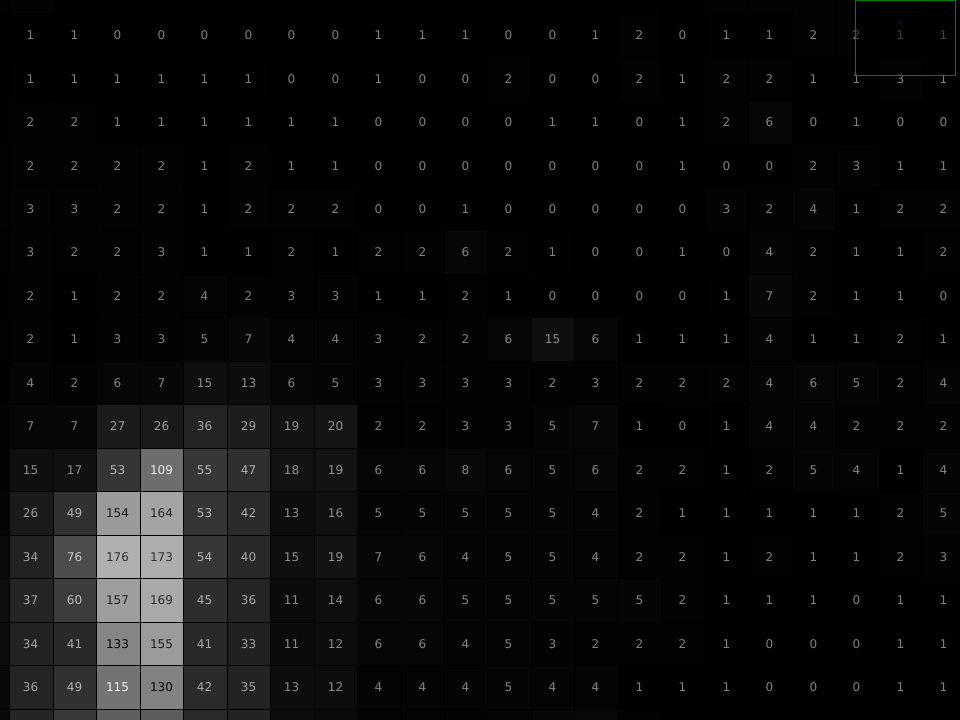
\includegraphics[width=0.75\linewidth]{img/hauptteil/bildverarbeitung/pixel_values_gray.png}
		\caption[Pixel-Werte im Grauwertbild]{Der selbe Ausschnitt wie in Abb. (\ref{fig:pix_values}), nur als Grauwertbild konvertiert.}
		\label{fig:pix_values_gray}
	\end{figure} 
	
	Die Abbildungen (\ref{fig:pix_values}) und (\ref{fig:pix_values_gray}) zeigen auch, dass eine Laserlinie bis zu 4 oder 5 Pixel breit sein kann. Für die Weiterverarbeitung soll sie allerdings nur eine Breite von einem Pixel haben. Dazu wird in jeder Pixel-Zeile in einem Bild nach der höchsten Intensität gesucht. Das ist jedoch nur sinnvoll, wenn die Laserlinie im Bild von oben nach unten geht. Der Laser muss demnach entsprechend zur Kamera angebracht werden. Diese Anforderung kann schon im Aufbau des Sensors beachtet werden. Im Kapitel \ref{chap:grundlegender_aufbau} wurde beschrieben, dass Kamera und Laser zueinander in der gleichen Position bleiben. Demnach kann der Laser entsprechend so angebracht werden, dass er im Kamerabild entsprechend aufgenommen wird.
	
	\subsubsection{Gauß-Filter}
	Die einfachste Methode wäre also jede Zeile nach der höchsten Intensität zu suchen und den betreffenden Pixel auszuwählen. Dieser Pixel befindet sich je nach Aufnahme jedoch nicht genau in der Mitte der Laserlinie. Die erarbeiteten Linien können so sehr \glqq wellig\grqq{} werden, da Pixel untereinander zum Teil stark in ihrer Position in der Zeile abweichen. Den Pixel mit der höchsten Intensität als Ausgangspunkt zu nehmen ist gut, jedoch sollen die umliegenden Pixel einen Einfluss machen können, um die Genauigkeit der Laserlinie zu erhöhen. Dazu wurden zwei Vorgänge entwickelt. \newline
	Die erste Methode ist es, einen Gauß-Filter über das Grauwert-Bild zu legen. Ein Gauß-Filter ist ein Weichzeichner, der umgangssprachlich ein Bild verwischt oder unscharf macht bzw. das Grauwertbild glättet \citep[vgl.][S. 134ff]{nischwitz_bildverarbeitung_2020}. Der Gauß-Filter wird auf jeden Pixel im Bild angewandt. Dabei ändert er den Wert des ausgewählten Pixels in Abhängigkeit der umliegenden Pixel. In diesem Projekt wird er dabei in einer Reichweite von einem 5x5-Feld definiert. Das bedeutet, dass ausgehend von dem ausgewählten Pixel ein 5x5-Feld betrachtet wird. Der Gauß-Filter ist ein Tiefpassfilter und wirkt damit möglichem Rauschen im Bild entgegen. Wenn ein einzelner Pixel ein hohen Wert aufweist, jedoch alle anderen um diesen herum im Vergleich niedriger sind, wird der Pixel-Wert nach der Filter-Operation niedriger ausfallen. So werden demnach vereinzelte Pixel mit hoher Intensität dunkler gemacht. Bei Gruppen von Pixeln werden die Intensitäten aneinander angepasst.
	
	\subsubsection{Das Erstellen von Subpixeln}
	Nachdem der Filter verwendet wurde, kommt die Operation, in der jede Zeile des Bildes nach dem Laserlinien-Pixel abgesucht wird. Hier wird zuerst der Pixel mit der höchsten Intensität gesucht. Dabei kann immer noch mehr  Genauigkeit erzielt werden, wenn man die Pixel links und recht neben dem Ausgewählten mit beachtet. So fließt nicht nur die Intensität als Auswahlkriterium ein, sondern auch die benachbarten Pixel der Laserlinie in dieser Zeile. Da die erschlossenen Pixel in 3D-Koordinaten umgewandelt werden und somit vom Bild und der Pixel-Darstellung getrennt werden, ist es nicht mehr notwendig nur ganze Zahlen zu verwenden. Die Werte können also auch Nachkommastellen haben und sogenannte Subpixel ergeben. Für dieses Errechnen des passenden Subpixel wurde ein Algorithmus erstellt, der wie folgt funktioniert:
	
	$\underline{1. \; Grenzwert}$
	
	Zuerst wird ein passender Grenzwert für die Intensität gesucht, um eine Grenze festzulegen, ab welchen Wert überhaupt ein Pixel gefunden werden soll. Wenn die maximale Intensität in einer Zeile unter dem gewählten Grenzwert liegt, wird diese übersprungen. Damit wird auch ungewolltes Rauschen entfernt, da eine Intensität, die so niedrig ist, nicht zur Laserlinie gehören kann. Ein im Vorhinein festgelegter Grenzwert ist dabei nicht ausreichend, da dieser nicht an das aktuelle Bild angepasst wäre. Bilder können unterschiedlich ausfallen und nicht wie gewollt auf den Grenzwert reagieren. So können zu viele oder zu wenig Zeilen übersprungen werden. Der Grenzwert soll genau auf das aktuelle Bild angepasst sein. Die Otsu-Methode ist ein Schwellenwertverfahren, welches genau den gewollten Wert liefern kann \citep[vgl.][]{otsu_tlreshold_nodate}. Dabei wird von einem Grauwertbild ein Histogramm erstellt. Dieses wird analysiert und ein passender individueller Grenzwert ausgegeben. Die höchste Intensität der aktuellen Zeile wird auf diesen geprüft. Wenn sie zu niedrig ist, ist auch die ganze Zeile zu dunkel und wird nicht als Teil der Laserlinie angesehen.
	
	$\underline{2. \; Einbeziehen \; der \; benachbarten \; Pixel}$
	
	Der Ausgangspunkt ist jetzt der Pixel mit der höchsten Intensität und dieser liegt über dem errechneten Grenzwert. Die benachbarten Pixel sollen jetzt in einen endgültigen Wert mit einbezogen werden. Um das zu erreichen, wird eine Parabel genutzt. Es gilt eine quadratische Funktion in der Form \( ax^2 + bx + c = I_x \), wobei \( I \) die Intensität und \( x \) die Position in der jeweiligen Zeile ist. Bei einem Bild, das beispielsweise 1920 Pixel breit ist, ist das ein Wert zwischen 0 und 1919. Die quadratische Funktion wird auf den ausgewählten Pixel und seine Nachbarn angewandt. Somit gilt:
	
	\begin{equation}
	\begin{aligned}
	ax^2 + bx + c &= I_x \\
	a(x+1)^2 + b(x+1) + c &= I_{x+1} \\
	a(x-1)^2 + b(x-1) + c &= I_{x-1} \\
	daraus \; folgt: \\
	\underbrace{\begin{pmatrix}
		x^2 & x & 1 \\
		(x+1)^2 & (x+1) & 1 \\
		(x-1)^2 & (x-1) & 1 
		\end{pmatrix}}_{\substack{X}} \underbrace{ \begin{pmatrix}
		a \\
		b \\
		c
		\end{pmatrix}}_{\substack{\vec{abc}}} &= \begin{pmatrix}
	I_x \\
	I_{x+1} \\
	I_{x-1}
	\end{pmatrix}
	\end{aligned}
	\label{eq:subpixel_x}
	\end{equation}
	
	Das Ziel ist es den Vektor \( \vec{abc} \) herauszufinden. Da die Intensitäten und die x-Werte bekannt sind, ist \( \vec{abc} \) die einzige Unbekannte und kann errechnet werden. Im nächsten Schritt soll das Maximum der Parabel herausgefunden werden. Sie befindet sich dort, wo die tatsächliche Intensität am höchsten ist. Dieser x-Wert befindet sich dann in den meisten Fällen zwischen zwei Pixeln. Um das Maximum zu finden wird die Nullstelle der Ableitung errechnet. Dafür gilt:
	
	\begin{equation}
	\begin{aligned}
	2a \cdot x + b &= 0 \\
	x &= \frac{-b}{2a}
	\end{aligned}
	\end{equation}
	
	\( b \) und \( a \) sind durch das Errechnen von \( \vec{abc} \) bekannt und ein Wert für \( x \) kann gefunden werden.
	
	In der Rechnung fällt auf, dass x für jede Zeile individuell ausgerechnet wird. Dabei ändert sich in (\ref{eq:subpixel_x}) die Werte für \( x \) und die Intensitäten. Hier kann man die Berechnung vereinfachen. Wählt man für \( x = 0\), entsteht die folgende Matrix:
	
	\begin{equation}
	X = \begin{pmatrix}
	0 & 0 & 1 \\
	1 & 1 & 1 \\
	1 & -1 & 1
	\end{pmatrix}
	\end{equation}
	
	Wenn \( \vec{abc} \) mit dieser Matrix und den individuellen Intensitäten berechnet wird, erhält man die Abweichung zu Mitte. Dabei ist die Mitte 0 und das entspricht dem ausgewählten Pixel mit der höchsten Intensität. Man errechnet eine Zahl zwischen -1 und 1. Diese wird mit der x-Position des Ausgangspixel in der Zeile verrechnet. Der Algorithmus wurde somit vereinfacht, da sich in jeder Rechnung nur der Intensitäten-Vektor ändert und immer die gleiche Matrix \( X \) gewählt werden kann.
	
	\begin{figure}[h]
		\centering
		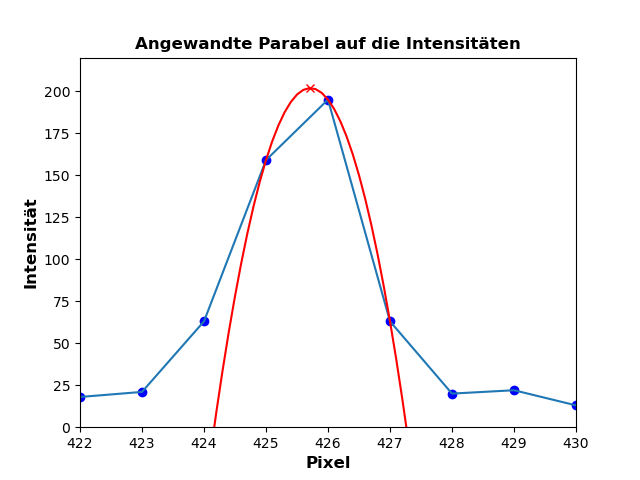
\includegraphics[width=0.7\linewidth]{img/hauptteil/bildverarbeitung/parable_intensities.png}
		\caption[Parabel für die Intensitäten]{Parabel für die Intensitäten. Die Blauen Punkte kennzeichnen einen Pixel und seine jeweilige Intensität. Die Parabel wird durch den Punkt mit der höchsten Intensität und seine Nachbarn gelegt.}
		\captionsource{Der gezeigte Ausschnitt stammt aus einer ausgewählten Zeile in Abb. (\ref{subfig:surface_diff})}
		\label{fig:parable}
	\end{figure} 
	
	Mit dem Finden des x-Wert ist die Bearbeitung einer Zeile fertig. Es gibt nun eine eindeutige 2D-Koordinate für einen Punkt der Laserlinie. Der Algorithmus geht über jede Zeile (y) und findet einen x-Wert. Dabei fügt er die gefundenen Subpixel (x, y) in einer Liste zusammen. Die Menge dieser Subpixel ist die Abbildung der Laserlinie in einen 2-dimensionalen Raum (Abb. (\ref{fig:pix_koord})). Diese wurde als Output gefordert.
	
	\begin{figure}[h]
		\centering
		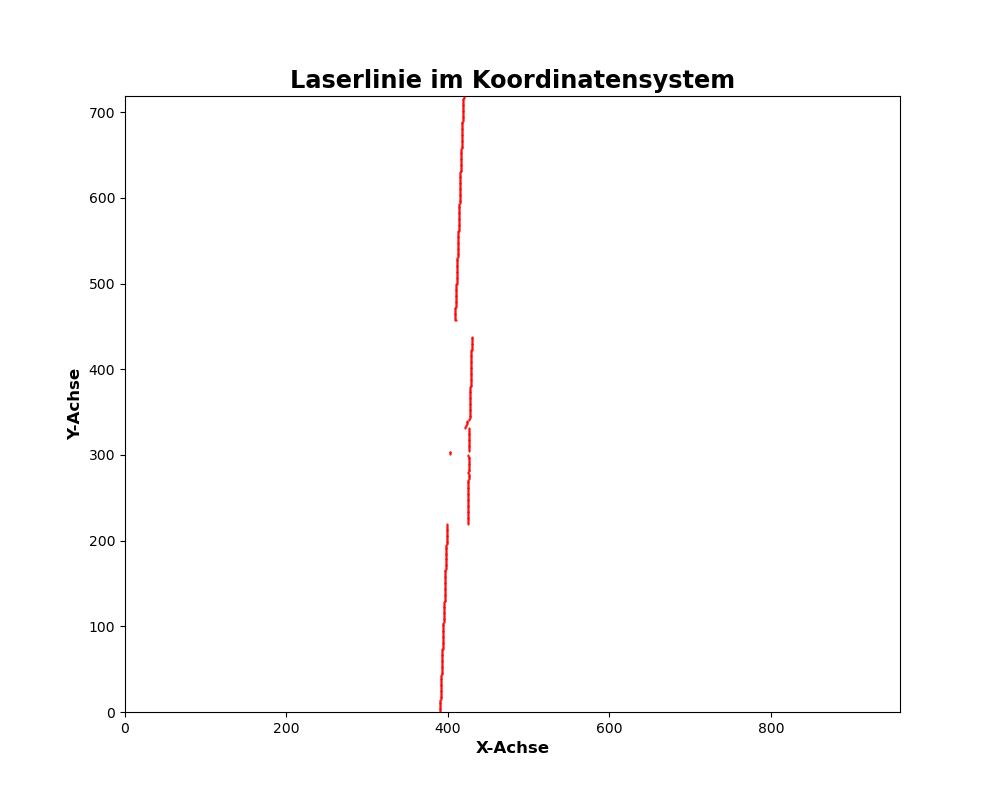
\includegraphics[width=0.8\linewidth]{img/hauptteil/bildverarbeitung/pixel_koord.png}
		\caption[Subpixel im Koordinatensystem]{Die Subpixel können nun in einem Koordinatensystem dargestellt werden.}
		\label{fig:pix_koord}
	\end{figure} 

	Wenn man die Abb. (\ref{fig:pix_koord}) und (\ref{subfig:surface_diff}) vergleicht, fällt auf, dass die Abbildung im Koordinatensystem gespiegelt ist. Das liegt daran, dass die Nummerierung der Pixel im Bild oben links beginnt (der Nullpunkt mit Pixel (0, 0)) und bei einem Koordinatensystem unten links. 

	\label{chap:erkennen_der_laserlinie}
